\subsection{Background}
Digital machinery launched into space is exposed to a number of
environmental hazards not normally encountered in operation on
earth. This includes dangers such as solar flares and strong cosmic
background radiation.\cite{nasa}

One way of coping with these problems is to introduce redundancy in
the system design by duplicating elements. For instance, instead of
using a single microprocessor to perform relevant calculations, one
might use four of them. This way the system can continue its operation
even in the face of failure in one or possibly even several of the
redundant components.

For a component to be of use in general, it will naturally have to
either produce some result to be consumed by another part of the
system or change the state of the system. Duplicating interal
components of the system will therefore have an impact on their
surroundings, since communicating entities will only accept data from
a single source. It is also undesirable to allow components which have
failed to change the system state.

There are several ways to tackle this design issue. One would be to
introduce redundancy in the components which communicates with the
duplicated component---if you duplicated a sensor, for instance, you
could also duplicate the processor it communicates with. Another
strategy would be to add other components which combines the output
from the duplicated components and sends this as input to the
peripheral unit.

\subsection{The Problem}
\label{sec:problem}
Our task was to design a system component, named the Liaison System,
which handled this problem by taking the latter
approach. Specifically, the Liaison System was to work in an
environment containing four microprocessor performing the same
computation. This environment is depicted in
\autoref{fig:systemenvironment}. 

\begin{figure}[H]
    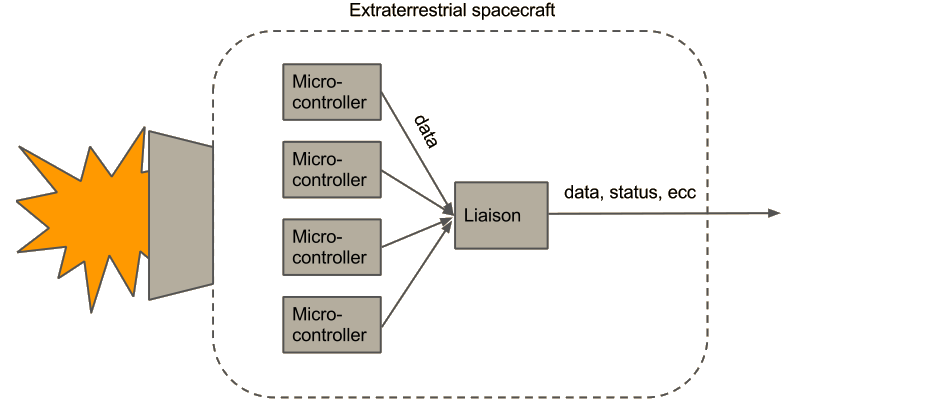
\includegraphics[width=15cm]{fig_system_env}
    \caption{The Liaison System Environment}
    \label{fig:systemenvironment}
\end{figure}

These microprocessors emit eight bit data words serially. The task of
the Liaison System was to perform a majority vote amongst the
microcontrollers assumed to work, and tag microcontrollers as broken
if their data differed from the majority.

The Liaison should also emit a status code after each majority eight
bit word, describing what failures it had observed in the system up to
this point. The status codes are listed in \autoref{tab:systemstatus}.

\begin{table}[htbp]
  \centering
  \begin{tabular}{|c|c|}
    \hline
    \textbf{Number of Failed Microcontrollers} & \textbf{Binary Status Code} \\ \hline
    0 & 000 \\ \hline
    1 & 001 \\ \hline
    2 & 010 \\ \hline
    3 or 4 & 111 \\ \hline
  \end{tabular}
  \caption{System status code given microcontroller failures.}
  \label{tab:systemstatus}
\end{table}

In addition to this, the Liaison should also be able to generate an
error correcting code which could be used to detect and repair a one
bit error and detect a two bit error in the data word and status. This
would be used to detect errors in the transmission. We were required
to use a Hamming code\cite{task}\cite{ecc}.

The Liaison was to be implemented using VHDL, and synthesized for the
Xilinx Virtex4 XC4VFX12-SF363-12 FPGA. The top level module of the
Liaison system was required to implement a specified VHDL entity
interface, listed in \autoref{apx:liaison}. It was also a requirement
that the {\ttfamily reset} should be synchronous. It was stated that the
design should focus on creating an area stringent a design as
possible. Specifically, the number of LUTs required on the FPGA after
synthesis should be minimized.

During the design of the Liaison system, we should consider several
alternatives and document their relative strengths and
weaknesses. Based on this investigation, we should choose the
alternative found to comply the best with our design goals. In this
report, we will first describe the design and implementation of our
final system. A discussion of alternatives is found in
\autoref{sec:discussion}.

Finally, in addition to designing the Liaison system, we should also
perform an evaluation of its expected lifetime. This evaluation should
consist of a calculation of the probability of an error in maximum one
controller, maximum two controllers or at least three controllers as a
function. We should also compute the mean time to failure for the
entire system, i.e. its expected lifetime.
